\chapter{Ontologie}
 
Pojem ontologie má dlouhou historii ve filozofii, kde představuje jako obor metafyziky nauku o podstatě existence a bytí jako takovém \cite{Dictionary}.
Ontologií se z filozofického hlediska zabýval například již Aristoteles \cite{gruber}.

Ontologií se však dnes zabývá také obor umělé inteligence a pro jeho účely se ontologie definuje z hlediska počítačové vědy.
Filozofické pojetí ontologie i její pojetí z hlediska počítačové vědy společně studuje entity a vztahy mezi nimi \cite{kunc}.
Ontologie se používají k zachycení znalostí nějaké domény (hudba, jídlo, cokoliv). Popisuje věci související s doménou a vztahy mezi těmito věcmi \cite{owltutorial}.
    
Pro informatické pojetí ontologie existuje hned několik definic, použijeme zde tu nejčastější, formulovanou duchovním otcem ontologie Tomem Gruberem; 
ontologie je "explicitní specifikace konceptualizace" \cite{gruber} či "formální specifikace sdílené konceptualizace" \cite{ontology}, kde jsou navíc vyřčeny požadavky na formálnost a sdílenost.

V počítačovém a informatickém kontextu ontologie definuje reprezentativní prvky pro modelování znalostní domény. 
Těmito prvky jsou obvykle třídy (či množiny), atributy (vlastnosti), a vzájemné vztahy mezi prvky třídami.
Tyto definované prvky zároveň obsahují informace o jejich významu \cite{gruber}.

Ontologie jsou hlavním pilířem Sémantického webu \cite{ontology}.

\section{Použití ontologií}

Noy a Mcguinness uvádějí důvody proč vytvářet ontologie, mezi nejdůležitější patří \textit{sdílení struktury informací mezi lidmi či softwarovými programy} a \textit{opakovaně použitelné znalostní domény} \cite{noy}.

S tím souvisí např. projekt Linked Data, který má za úkol propojit související webový obsah, který byl v minulosti vytvořen bez vzájemných spojení. Linked Data popisuje doporučený způsob jakým sdílet a spojovat informace a znalosti v rámci Sémantického webu \cite{linkedData}.
Aktuální sít vzájemně propojených ontologií ukazuje obrázek \ref{img:linkeddata}.

\section{Struktura ontologie}

Struktura ontologií je dána způsobem její reprezentace - nejčastějším způsobem se ontologie zapisují pomocí ontologického jazyka \ref{chapter:ontologyLanguage}.
Nicméně všechny způsoby reprezentace jsou si podobné. Běžně se tedy ontologie zkládají z těchto komponent \cite{noy}:

\begin{itemize}
\item Třídy (někdy nazývané také koncepty, množiny) - Základní stavební blok ontologie.
\item Atributy - Definují vlastnosti a charakter každé třídy.
\item Instance (objekty, individua) - Jsou instancemi tříd. Ontologie společně s množinou instancí vytvářejí znalostní bázi.
\item Relace (vztahy) - Udává souvislosti mezi třidami a instancemi.
\item Podtřídy - Blíže popisují rodičovskou třídu.
\item Axiomy - Logické formule.
\end{itemize}

\textit{Třídy} jsou základem ontologií, dávají jim strukturu. Uvažujme například doménu filmu - hlavní třída bude film. Můžeme tedy vytvořit podtřídy jako např. sci-fi, horor a komedie. Třída horor bude dále rozdělena na psycho a krvelačný. Každá podtřída tak blíže charakterizuje rodičovskou třídu. Schéma takové domény je znázorněno na obrázku \ref{img:movieClasses}.

\begin{figure}[h]
\begin{center}
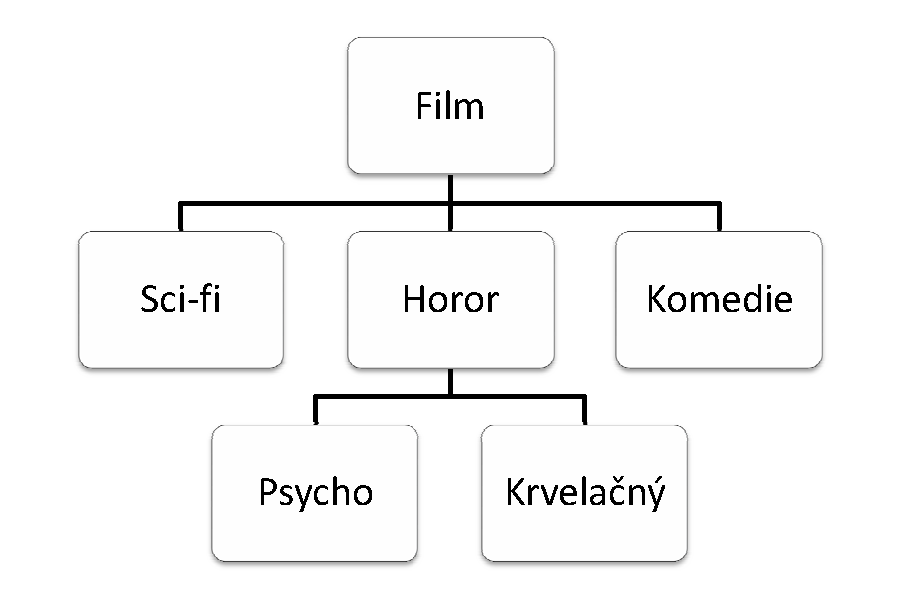
\includegraphics{figures/movieClasses}
\caption{Příklad hierarchie tříd v ontologii domény filmu.}
\label{img:movieClasses}
\end{center}
\end{figure}

\textit{Instance} odpovídá konkretnímu objektu reálného světa. Zda určitý objekt považovat za instanci či třídu není však čistě objektivní, závisí na konkrétním využití ontologie \cite{ontowww}.

\textit{Axiomy} jsou pravidla, které je možné do ontologie přidávat. Vyjadřují např. ekvivalenci a disjunkci tříd.

\section{Vytváření ontologie}

V této sekci si ukážeme, jak se taková ontologie připravuje.

\subsection{Ontologie vína}

Třídy utvářejí představu o doméně. Například třída vín reprezentuje všechna vína.
Konkrétní vína jsou instancemi tříd těchto vín, tedy např. Bordeaux víno je instancí třídy "Bordeaux vína".
Třídy mohou mít podtřídy, kde každá podtřída blíže specifikuje rodičovskou třídu.
V našem příkladu můžeme třídu všech vín rozdělit na podtřídy červené, bílé a růžové (nebo také na suché, polosuché, polosladké, sladké či na perlivé, šumivé, stolní...) \cite {noy}.

Atributy popisují vlastnosti tříd a instancí. Château Lafite Rothschild Pauillac je vyráběn v Château Lafite Rothschild vinici (viz obr. \ref{img:wine}).
Máme tedy atribut vína "výrobce" s hodnotou Château Lafite Rothschild vinice.
Na úrovni tříd můžeme říci, že instance třídy Víno budou mít atributy pro vyjádření příchuti, obsahu cukru, výrobce atp. 

Atributy "výrobce" všech instancí třídy Víno, včetně její podtřídy Pauillac, mají jako hodnotu instanci třídy Vinice (viz obr. \ref{img:wine}).
Všechny instance třídy Vinice mají vlastnost "vyrábí", která ukazuje na všechny vína (= instance třídy Víno a její podtřídy), která daná vinice vyrábí.

Vývoj ontologie obsahuje kroky:

\begin{itemize}
\item Definování třid ontologie.
\item Taxonomické uspořádání tříd (vytvoření hierarchie).
\item Definování atributů a jejich dovolených hodnot.
\item Naplnění instancí a atributů konkrétními hodnotami.
\end{itemize}

\begin{figure}[h]
\begin{center}
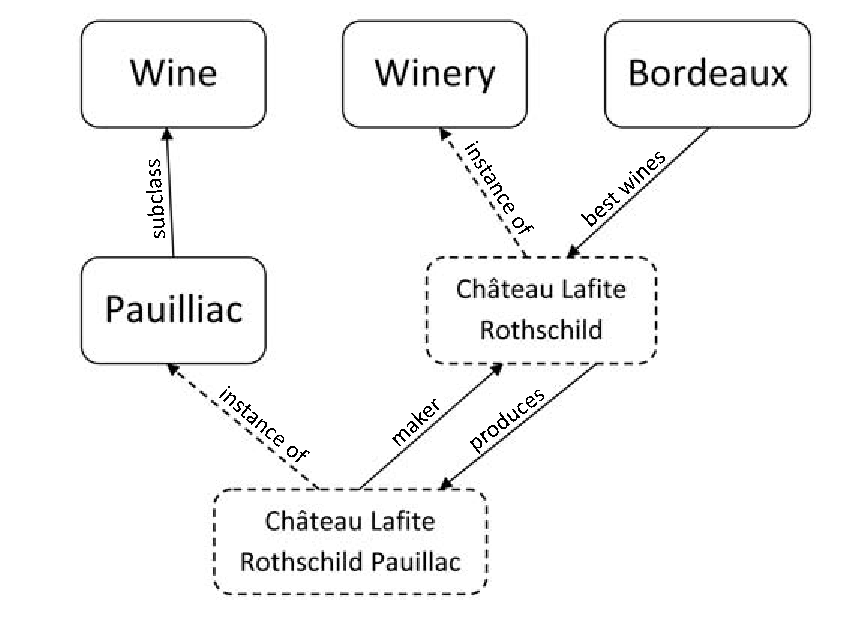
\includegraphics{figures/wine}
\caption{Ukázka ontologie vína resp. některých tříd a vazeb mezi nimi. Čárkované boxy představují instance, ostatní boxy značí třídy. Šipky značí jednotlivé vztahy.}
\label{img:wine}
\end{center}
\end{figure}

Další podrobnější příklad vytváření ontologie uvádí \cite{owltutorial} jako ontologii Pizzy \cite{pizza}.

\section{Jazyky ontologie}
\label{chapter:ontologyLanguage}

Každá ontologie, aby mohla být strojově čitelná, musí být zapsána formálně, pomocí jazyka. Takový jazyk se nazývá jazykem ontologie. 
Ontologické jazyky umožňují tvůrcům ontologií jednoznačně a formálně popsat konceptualizaci, tj. systém pojmů modelující určitou část světa. 
Hlavní požadavky na tyto jazyky jsou \cite{staab}:

\begin{itemize}
\item správně definovaná syntaxe
\item vhodná podpora dedukce 
\item formální sémantika
\item adekvátní výrazové schopnosti
\end{itemize}

Formální sémantika zajišťuje správně vyjádření znalostní struktury. Umožňuje různým lidem či zařízením stejnou interpretaci ontologie. 
Umožňuje na základě znalostí vyvozovat závěry. K tomu napomáhají i následující tvrzení \cite{staab}:
\begin{itemize}
\item Členství ve třídě - Jestliže x je instance třídy B a B je podtřídou třídy A, potom můžeme tvrdit, že x je instancí třídy A.
\item Ekvivalence tříd - Jestliže třída A je ekvivalentní s třídou B a třída B je ekvivalentní s třídou C, poto je třída A ekvivalentní s třídou C.
\item Konzistence tříd - Jestliže jsou dvě třídy disjunktní, podtřída obou těchto tříd bude prázdná.
\item Klasifikace tříd - Mějme definované vlastnosti třídy A, pak můžeme tvrdit: Pokud instance x má stejné vlastnosti, je tato instance x instancí třídy A.
\end{itemize}

Výrazová schopnost jazyka se volí podle účelu nasazení. Čím větší vyjadřovací schopnosti jazyk ale má, tím více se stává složitějším pro počítače.
Např. v jazyce OWL existují hned tři úrovně výrazovosti (OWL Lite, OWL DL, OWL Full). 
U jazyka OWL Full je už pro počítač mnohdy složité dopočítat se výsledku.

    \subsection{Resource Description Framework}
        
        Jedním z pilířů Sémantického webu je technologie Resource Description Framework (RDF) \cite{semWeb}, 
        jedná se o jazyk reprezentující informace o zdrojích ve webovém prostředí \cite{RDFprimer}, umožňuje výměnu a sdílení znalostí na webu \cite{RDF}.
        
        RDF nám umožňuje pracovat s informacemi na webu, namísto pouhého zobrazení dat uživateli. Díky RDF totiž počítač těmto datum rozumí, např. jméno osoby chápe jako skutečné jméno a ne jen jako pouhý shluk písmen. Jednotlivé aplikace tak mohou s informacemi pracovat a sdílet mezi sebou. 
        
        RDF je založeno na identifikaci všech věcí pomocí webových identifikátorů Uniform Resource Identifiers (URI). Popisuje informace jednoduše pomocí klíče:hodnoty, resp. vlastnosti a její hodnoty. Díky tomu může RDF jednoduše zobrazit informace jako graf uzlů a hran reprezentující zdrojová data \cite{RDFprimer}.
        
        Např. Eric Miller je jako osoba definována http://www.w3.org/People/EM/contact\#me, která má dále email a titul. RDF graf tohoto příkladu uvádí obr. \ref{img:miller}.
        
        \begin{figure}[h]
        \begin{center}
        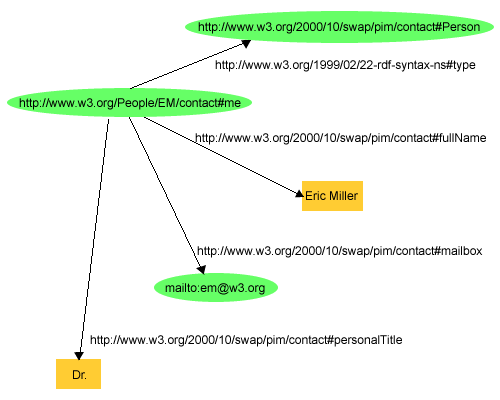
\includegraphics[width=11cm]{figures/rdf}
        \caption{RDF graf popisující osobu Eric Miller. (Zdroj \cite{RDFprimer})}
        \label{img:miller}
        \end{center}
        \end{figure}

        Další způsob reprezentace RDF je vedle grafu tzv. trojice. V troj-notaci je každý výrok zapsán jako trojice \textit{podmět, predikát, předmět} (v tomto pořadí). 
        Např. výrok "Osoba se jmenuje Eric Miller" z příkladu \ref{img:miller} se zapíše jako:
        
        \begin{verbatim}
        http://www.w3.org/People/EM/contact#me 
        http://www.w3.org/2000/10/swap/pim/contact#fullName 
        http://www.w3.org/2000/10/swap/pim/contact#mailbox
        \end{verbatim}
        Předchozí trojice by měla být zapsána do jednoho řádku, pro lepší přehlednost zde však uvádíme v řádcích.
        
        \subsubsection{Resource Description Framework in attributes} 
        
        Resource Description Framework in attributes (RDFa) je další W3C\footnote{World Wide Web Consortium (W3C) je hlavní standardizační organizace pro WWW.} specifikace.
        RDF je v praxi oddělený, samostatný soubor, sloužící jen pro webovou aplikaci, zatímco uživateli je nabídnuta XHTML stránka. 
        RDFa oproti tomu umožňuje vkládat RDF trojice přímo do XHTML dokumentů a tím tak podobně jako mikroformáty obohacují data o metadata \cite{RDFa}.
        
        \subsubsection{Resource Description Framework Schema}
        
        Resource Description Framework Schema (RDFs) je sémantickým rozšířením jazyka RDF.
        RDFs je nadstavbou RDF, doplňuje třídy a možnost stanovit definiční obor a obor hodnot. RDFs umožňuje zachycení sémantiky obsahu stránek \cite{ontowww}.
        
        \subsubsection{RDF/XML}
        
        RDF/XML je serializace RDF grafů do XML syntaxe \cite{rdfxml}. 
    
    \subsection{SPARQL Protocol and RDF Query Language}
    
    SPARQL Protocol and RDF Query Language (SPARQL) - název je rekurzivní zkratka - je další klíčovou technologií Sémantického webu \cite{sparqlwiki}.
    SPARQL je, jak vyplývá z názvu, dotazovací jazyk pro RDF. Vyhledává množiny trojic, které vyhovují zadanému dotazu.   
    Výsledkem SPARQL dotazu je opět trojice či množina trojicí podmět, predikát, předmět.
    
    Vzorový SPARQL dotaz:
    
    \begin{verbatim}
    PREFIX abc: <http://example.com/exampleOntology#> 
    SELECT ?capital ?country
    WHERE {
      ?x abc:cityname ?capital ;
         abc:isCapitalOf ?y .
      ?y abc:countryname ?country ;
         abc:isInContinent abc:Africa .
    }
    \end{verbatim}
    
    vrátí množinu trojic:
    
    \begin{verbatim}
    ?capital http://example.com/exampleOntology\#isCapitalOf ?country
     \end{verbatim}
     
     Jinými slovy vráti seznam všech zemí a jejich hlavních měst v Africe.
        
    \subsection{Ontology Web Language}

    Ontology Web Language (OWL) vznikl pod záštitou W3C a vychází z DAML+OIL ontologického jazyka \cite{owlguide}.
    Je dalším jazykem pro vytváření ontologií a rozšiřuje vyjadřovací schopnosti jazyka RDF resp. přidává mu další sémantickou vrstvu. \cite{semWebStandards}.
    Má např. bohatší sadu operátorů (and, or, negace) \cite{owltutorial}a zavádí disjunktní třídy a kardinalitu vztahu \cite{staab}. 
    Vyjadřovací schopnosti naznačuje obrázek \ref{img:owlexpressiveness}
    
    \begin{figure}[h]
    \begin{center}
    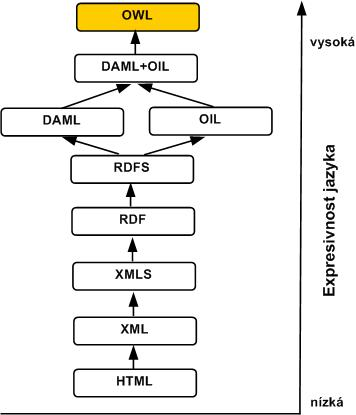
\includegraphics[width=8cm]{figures/owlexpressiveness}
    \caption{Vyjádření expresivnosti OWL jazyka. (Zdroj \cite{owlhradec})}
    \label{img:owlexpressiveness}
    \end{center}
    \end{figure}
        
        \subsubsection{Dialekty OWL}
        
            OWL ontologie byly vyvinuty ve třech verzích (syntaktických podmnožinách), a to OWL-Lite, OWL-DL a OWL-Full lišící se svoji vyjadřovací schopností \cite{owlguide}:
            
            \begin{itemize}
            \item \textbf{OWL Lite} má nejmenší vyjadřovací schopnosti. 
            Je navržen pro použití v situacích, kde stačí jednoduchá hiearchie tříd a jsou požadovány jen jednoduché omezení (např. kardinalita pouze 0 či 1).
            
            \item \textbf{OWL DL} nabízí vysokou míru vyjadřovacích schopností s garancí vypočítatelnosti (vždy se lze dobrat výsledku v konečném čase). 
            OWL DL je založena na deskripční logice (odtud zkratka DL). 
            Deskripční logika vychází z predikátové logiky, je ale omezenější \cite{svatek}.
            
            \item \textbf{OWL Full} obsahuje kompletní vyjadřovací sílu a plnou syntaxi RDF Schema, díky čemuž ale není garantována vypočítatelnost (dobrání se výsledku). 
            \end{itemize}
            
            Každý z výše popsaných podjazyků je rozšířením svého jednoduššího předchůdce, tzn. každá syntakticky správná OWL Lite ontologie je zároveň správnou OWL DL ontologií a každá správná OWL DL ontologie je OWL Full ontologií.
            Stejný princip platí i u vyvozování těchto ontologií.
            
        \subsubsection{Komponenty OWL}
            
            Mezi základní kompomenty OWL jazyka patří \cite{owltutorial}:
            
            \begin{itemize}
            \item \textbf{Individua (instance)} - Individua reprezentují skutečné objekty v rámci domény, kterou se zabýváme. Jedná se o instance tříd.
            Příklad znázornění instancí ukazuje obrázek \ref{img:individuals}.
            
            \begin{figure}[h]
            \begin{center}
            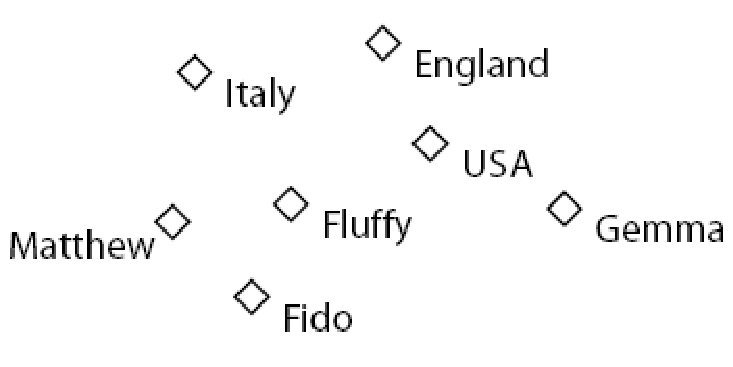
\includegraphics[width=10cm]{figures/individuals}
            \caption{Příklad instancí. (Zdroj \cite{owltutorial})}
            \label{img:individuals}
            \end{center}
            \end{figure}
            
            \item \textbf{Vlastnosti} - Vlastnosti se používají k definici vztahu mezi dvěma objekty (individui). Mohou mít inverze, mohou bít funkční (tj. mohou mít pouze jednu hodnotu), tranzitivní\footnote{Mějmě vlastnost T a instance a,b,c. Vlastnost T je tranzitivní, jestliže a T b a zároveň b T c, potom platí i a T c. Zdroj \cite{relace}} a symetrické\footnote{Mějme vlastnost S a instance a,b. Vlastnost S je symetrická, pokud platí a S b a zároveň b S a. Zdroj \cite{relace}}.
            Obrázek \ref{img:properties} představuje instance a jejich vztahy (vlastnosti).
            
            \begin{figure}[h]
            \begin{center}
            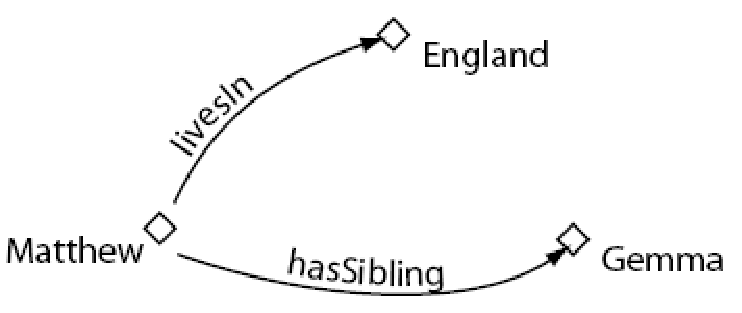
\includegraphics[width=10cm]{figures/relations}
            \caption{Příklad vztahů mezi individui. (Zdroj \cite{owltutorial})}
            \label{img:properties}
            \end{center}
            \end{figure}
            
            
            \item \textbf{Třidy} - Můžeme si je představit jako množiny obsahující individua, které spolu sdílejí některou vlastnost.
            Obrázek \ref{img:classesindividuals} vyjadřuje několik tříd obsahující instance (kde některé instance mají mezi sebou vztah). 
            
            \begin{figure}[h]
            \begin{center}
            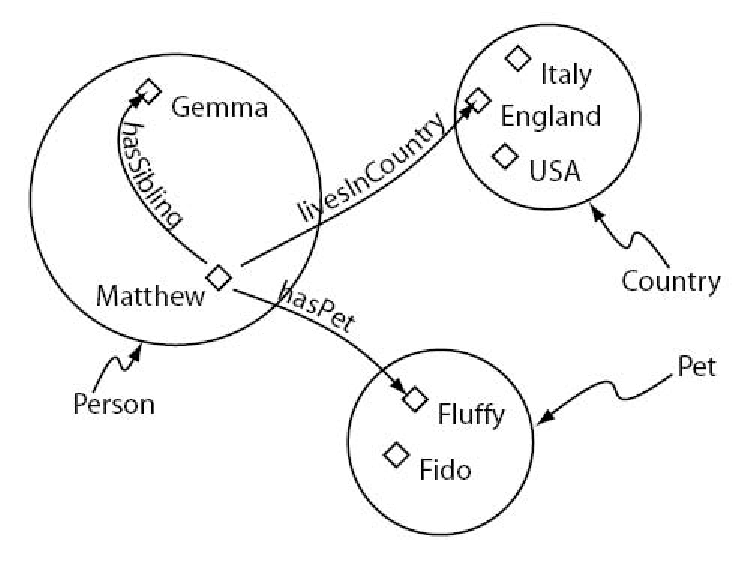
\includegraphics[width=10cm]{figures/classes}
            \caption{Příklad tříd s instancemi. (Zdroj \cite{owltutorial})}
            \label{img:classesindividuals}
            \end{center}
            \end{figure}
            
            \end{itemize}
            
        \subsubsection{OWL 2}  
            
        OWL2 je ontologický jazyk Sémantického webu, který schválila skupina W3C jako své doporučení v říjnu 2009. Nahrazuje a rozšiřuje původní OWL jazyk z roku 2004 (zpětně označovaného jako OWL 1), se kterým je zpětně kompatibilní. Jazyk je stále založen na RDF a původní OWL 1 doplňuje např. o klíče, řetezení vztahů, bohatší datové typy, dále přidává možnost asymetrických a disjunktních vztahů.
        Obrázek \ref{img:owl2} ukazuje základní stavební bloky a jejich propojení. Elipsa představuje abstraktní notaci ontologie (může být buď jako abstraktní struktura či jako RDF graf). Nahoře jsou konkrétní varianty syntaxe, které OWL 2 může používat k serializaci ontologie. Dole pak jsou dvě sémantické specifikace definující význam OWL 2 ontologií.
        Jako hlavní serializaci OWL 2 používá RDF/OWL \cite{owl2}.
       
        \vspace*{6pt}
        \textbf{Dialekty a Profily OWL 2}
        \vspace*{6pt}
       
        OWL 2 definuje dva podjazyky OWL 2 DL a OWL 2 Full.
        Dále definuje OWL 2 Profily jako podjazyky (syntaktické podmnožiny) jazyka OWL 2. Jsou definovány tři profily: OWL 2 EL, OWL 2 QL a OWL 2 RL definované opět jako syntaktické podmnožiny OWL 2. Každý z profilů je více restriktivní než jazyk OWL 2 DL \cite{owl2primer}. 
        
        OWL 2 Profily \cite{owl2primer}:
        
        \begin{itemize}
        \item \textbf{OWL 2 EL} je podobný OWL 2 DL s některými omezeními. Zkratka EL značí tzv. EL deskripční logiku\footnote{EL je malá deskripční logika \cite{EL}}.
        
        \item \textbf{OWL 2 QL} může být realizován použitím standartních relačních databázových technologií jako je např. Structured Query Language (SQL). Díky tomu může být pevně sloučen s Relational database management system (RDBMS). Zkratka QL tedy značí Query Language.
        
        \item \textbf{OWL 2 RL} je určen pro aplikace vyžadující různou škálu logického usuzování (reasoning) bez přílišného obětování vyjadřovací síly.
        \end{itemize}
        
        \subsubsection{OWL/XML}
        
        Obdobně jako RDF/XML je OWL/XML serializací OWL ontologie do XML syntaxe \cite{owlxml}.
        
\section{Analýza nástrojů na tvorbu ontologií}

\subsection{Editor ontologií}
Pro navrhování a modelování ontologií potřebujeme vhodný nástroj pro editaci ontologií, težko budeme ontologii vytvářet čistě v textovém editoru (teoreticky to však samozřejmě při dobré znalosti konkrétní syntaxe lze).

Nejpoužívanějším editorem ontologií je \textit{Protégé}\footnote{Protégé \url{http://protege.stanford.edu/} vyvíjený v rámci projektu CO-ODE \url{http://www.co-ode.org/}.}, vytvořený na Standford University jako open-source \cite{owl2primer}.
Díky jeho otevřené formě lze do Protégé doplňovat nejrůznější zásuvné moduly (za všechny např. plugin OWL Wiz vizuálně znázorňující strukturu ontologie).
Protégé umožňuje exportovat vymodelovanou ontologii do různých syntaxí (např. RDF/XML, OWL/XML, OWL functional, Manchester OWL, turtle).

Dalším open-source nástrojem je \textit{SWOOP}\footnote{SWOOP \url{http://code.google.com/p/swoop/}} podobný Protégé. Dovede např. přehledně zobrazit syntaxi jen pro vybrané prvky ontologie, a to současně v abstraktní syntaxi, RDF/XML a Turtle syntaxi.

Poslední zmíním velmi povedený editor \textit{NeOn Toolkit}\footnote{NeOn Toolkit \url{http://www.neon-toolkit.org/}} postavený na Eclipse platformě, který také umožňuje přidání velkého množství zásuvných modulů.

K vytvoření hudební ontologie pro tuto práci budeme používat editor Protégé 4.0, a to z důvodu jeho rozšířenosti, podpoře exportu do různých syntaxí a vizualizačního pluginu.

\subsection{Programovací prostředí}

S vymodelovanou ontologií chceme dále pracovat, použít ji ve vhodné aplikaci, proto musíme v závislosti na programovacím jazyku zvolit vhodný nástoj, který mám s implementací pomůže. 
Naštěstí pro tyto účely dnes existuje spousta nástrojů \cite{semwebtools}.

Pro programovací jazyk Java je zřejmě nejrozšířenější nástroj \textbf{Jena Semantic Web Framework}\footnote{Jena Semantic Web Framework \url{http://jena.sourceforge.net/}}, který poskytuje programovací prostedí pro RDF, RDFS, OWL a SPARQL.

Pro PHP: Hypertext Preprocessor (PHP) prostředí existují tři hlavní nástroje, ARC, RAP, a Triplify \cite{semwebwikitools}:

\begin{itemize}
\item \textbf{ARC}\footnote{ARC \url{http://arc.semsol.org/}} (resp. ARC2) je open-source flexibilní RDF systém pro sémantický web postavení na PHP. Obsahuje několik RDF parserů (RDF/XML, Turtle, RSS, mikroformáty, RDFa atd.) a serialuzuje např. do RDF/JSON, RDF/XML a Turte. ARC dále pracuje se SPARQL dotazovacím jazykem. 
S RDF daty pracuje přes RDF Store pomocí MySQL databáze. 
RDF Store je systém pro ukládání a správu RDF dat \cite{rdfstore}. 

\item \textbf{RAP}\footnote{RAP \url{http://www.seasr.org/wp-content/plugins/meandre/rdfapi-php/doc/index.html}} je RDF API pro PHP. RAP je systém pro parsování, dotazování, manipulaci, serializaci a obsluhu RDF. 

\item \textbf{Triplify}\footnote{Triplify \url{http://triplify.org/}} je plugin pro webové aplikace, který relační databázi transformuje do RDF či do JavaScript Object Notation (JSON) podoby a z databáze tak díky tomu vytváří sémantickou strukturu.
\end{itemize}

Seznam dalších nástrojů i pro jiné programovací jazyky (jako např. Python, C, C++, C\#, Perl, Ruby, Flex atd.) nabízí \cite{semwebtools}.

Pro tento projekt použijeme ARC systém (důvody proč právě ARC uvádím v následující kapitole \ref{chapter:webappdesign}).  